
\section{Involved Technologies}

\subsection{JENA Ontology API}
There are several languages available for representing ontology information on the semantic web. They range from the most expressive, OWL Full, through to the weakest, RDFS. With RDFS it is possible to build a simple hierarchy of concepts, and a hierarchy of properties. The ontology language used in this project is the OWL FULL. OWL language allows properties to be denoted as transitive, symmetric or functional, and allows one property to be declared as the inverse of another.\\
\\
The Jena ontology API is a Java programming toolkit. Jena's support is limited to ontology formalisms built on top of RDF. One of the key benefits of building an ontology-based application is using a reasoner to derive additional truths about the concepts you are modelling. Jena includes support for a variety of reasoners through the inference API.
\\
A common feature of Jena reasoners is that they create a new RDF model which appears to contain the triples that are derived from reasoning as well as the triples that were asserted in the base model. The ontology API can query an extended inference model and extract information not explicitly given.

\subsection{ROS Famework}
The Robot Operating System (ROS) is a framework  for writing robot software. It is a collection of tools, libraries and conventions that aims to simplify the task of creating complex and robust robot behavior across a wide variety of robotics platforms. 
ROS was built from the ground up to encourage collaborative robotics software development. A ROS system consists of a large number of modules that pass data to one another using a inter-process communication. Each node sends and receives information to and from other nodes of the system using \textit{Topics}.
\\
\begin{figure}[H]
\centering
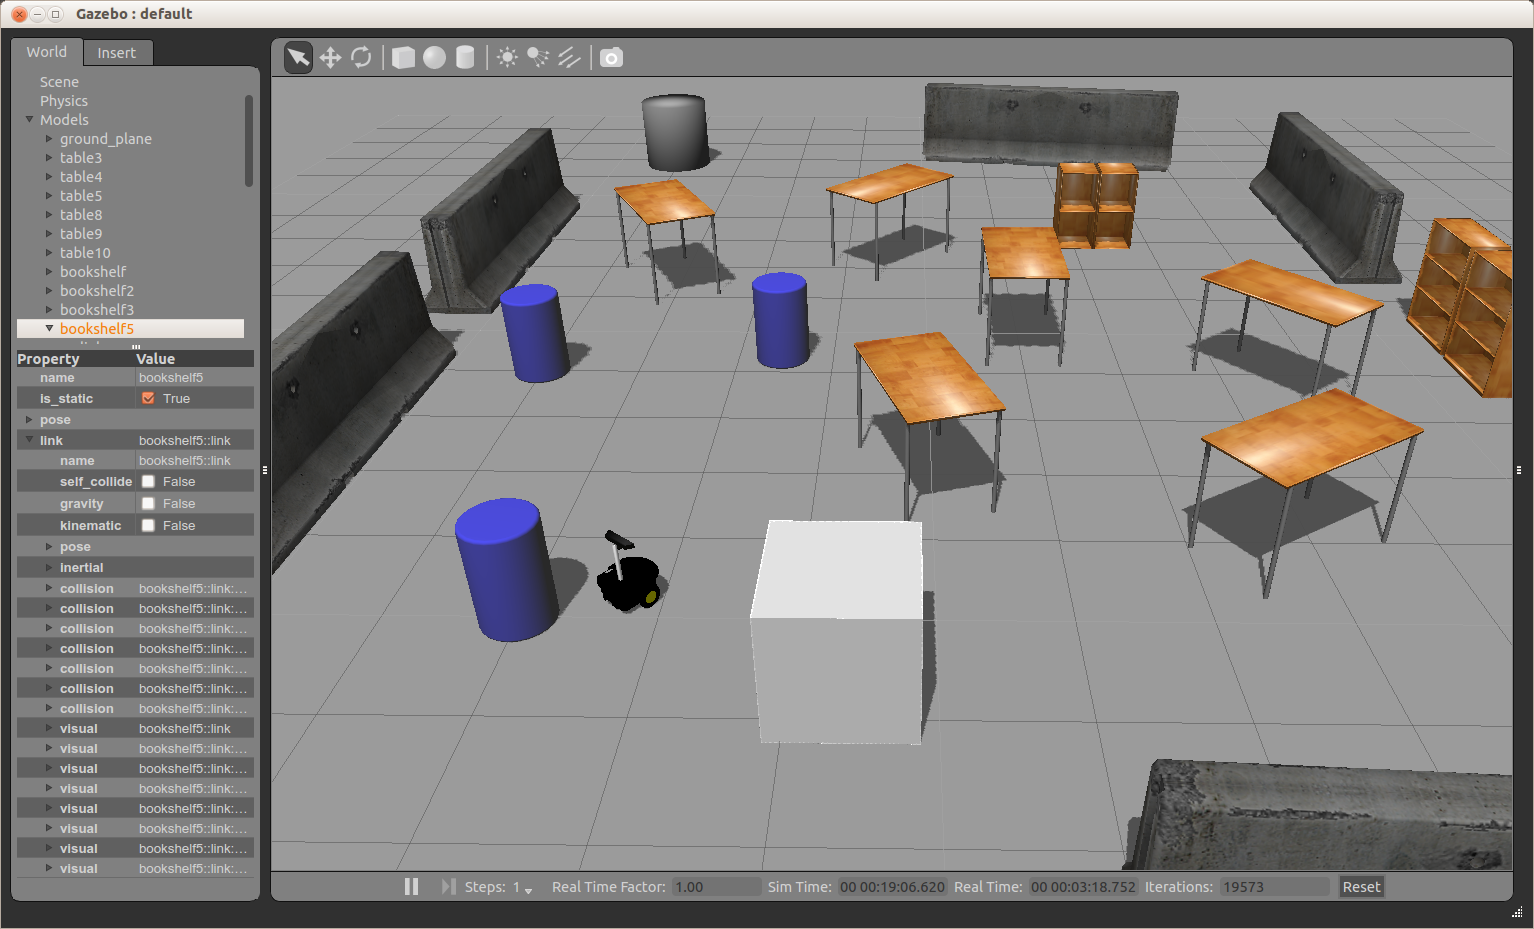
\includegraphics[width=0.8\textwidth]{imgs/gazebo1.png}
\label{fig:gazebo1}
\caption{ROS simulation}
\end{figure}

It is a tools-based program. Tasks such as visualizing the system interconnections generating documentation, logging data, filtering sensor's data, etc. are all performed by separate programs. The individual tools themselves are relatively small and generic. There is no central routing service.
\\
ROS chose a multilingual approach that allows programmers to accomplish tasks using scripting languages such as Python and MATLAB or using faster ones like C++. Client libraries exist for LISP, Java, JavaScript, Ruby,R and others. ROS libraries communicate with one another by following a convention that describes how messages are serialized before being transmitted over the network. The ROS conventions encourages contributors to create standalone libraries in order to allow the reuse of software and speed up development.\\
\\
The core of ROS is released under the BSD license which allows commercial and noncommercial use.

\subsection{Gazebo Simulation Environment}

Robotics implies robots. Most part of these platforms are used for research purposes and are custom built to investigate a particular aspect of interest. However, there are a growing number of standard products that can be purchased and used out of the box for development and operations in many domains of robotics.\\
Although several robotics platforms are considered to be low cost they are still significant investments. Even the best robots can break periodically due to various combinations of operator error, environmental conditions, manufacturing and design defects. All of these drawbacks can be avoided, or at least minimized, by using simulated robotic structures and a simulation environment. Gazebo is a $3D$ dynamic simulator with the ability to accurately and efficiently simulate populations of robots in complex indoor and outdoor environments. It offers physics engine with high degree of fidelity and a variety of sensors.

Many robots are provided including $PR2$, $Pioneer2$ DX, iRobot Create, TurtleBot and even champions of DARPA robotics challenge are available. Thanks to URDF format, robotics platforms can be created from scratch and deployed into the simulator.
With this environment it is possible to run simulation on remote servers, and interface to Gazebo through socket-based messages.

\begin{figure}[H]
\centering
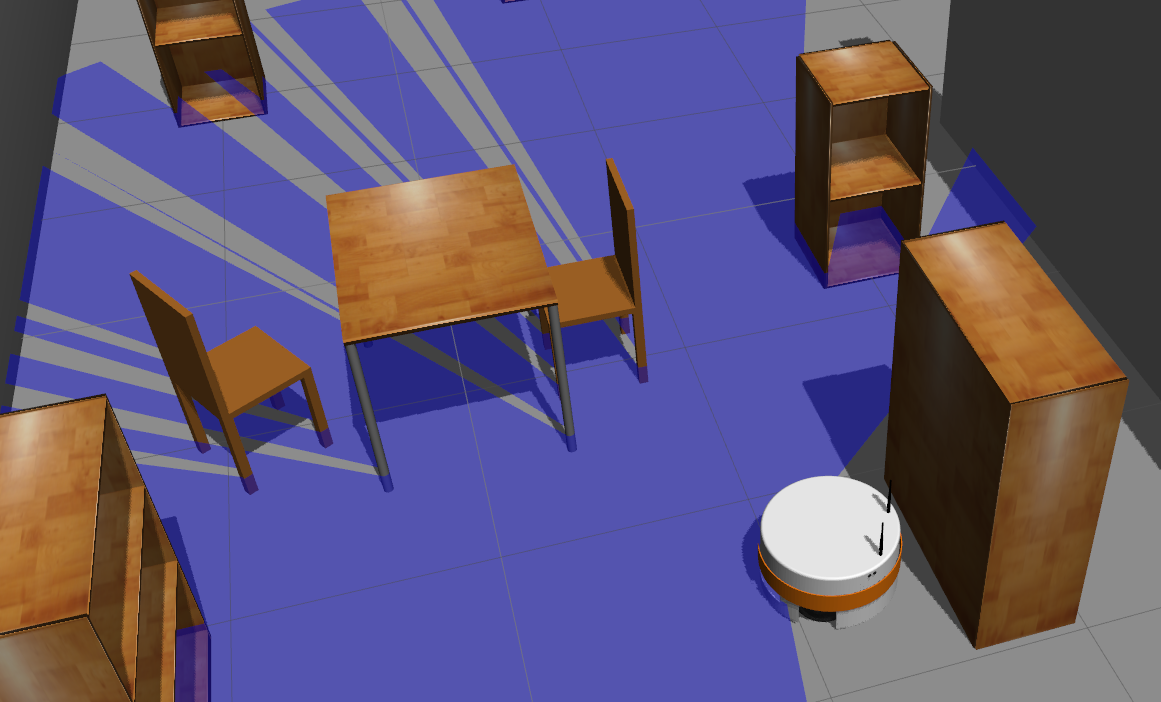
\includegraphics[width=0.5\textwidth]{imgs/gazebo2.png}
\label{fig:gazebo2}
\caption{Gazebo Environment}
\end{figure}

Ros integrates closely with Gazebo through the $gazebo\_ros$ package. The latter provides a Gazebo plugin module that allows bidirectional communication between ROS and the simulator. Sensors, physics data, video input can stream from Gazebo to ROS and actuators commands can be forwarded to the simulation environment. By choosing consistent names and data types for these data streams it is possible to run the low level device-driver software on both the real robot and in the simulator. In this project Gazebo 8.0 and ROS Indigo have been used. This combination ensures the compatibility required to flawlessly run the application.